%Do not change 
\documentclass[12pt, oneside]{article}
\usepackage{amssymb,amsmath}
\usepackage[margin=1in]{geometry}
\usepackage{textpos}
\usepackage{float}
%\usepackage{color}
\usepackage{graphicx}
\usepackage{tikz}
\usetikzlibrary{positioning}
\usepackage{tikz-3dplot}
\usepackage{pgfopts}
\usepackage{wasysym}
\usepackage{structuralanalysis}
\usepackage{fancyhdr}
\usepackage[en-US]{datetime2}

\fancyhead[R]{\small Last Updated: \today\ at \DTMcurrenttime}
\pagestyle{fancy}

% You may add the packages you need here



\begin{document}
% Do not modify 


%Do not modify
\begin{textblock*}{4cm}(-1.7cm,-2.3cm)
\noindent {\scriptsize AE737 Spring 2016} 
\end{textblock*}

%Do not modify other than putting your name where stated
\begin{textblock*}{8cm}(12.5cm,-1cm)
\noindent {Name: } 
\end{textblock*}
%Do not modify other than typing your acknowledgement where stated
\begin{textblock*}{13.5cm}(-1.7cm,-1.8cm)
%\noindent \textit{\footnotesize Acknowledgement: Your acknowledgement for collaboration and other sources goes here. } 
\end{textblock*}

\vspace{1cm}

%Do not modify other than typing the homework number after #
\begin{center}
\textbf{\Large Homework 5}

\textbf{Due 1 Mar 2016}
\end{center}


%Rest should contain your solution for the homework. Feel free to improvise in ways that you believe make grading easier.
\begin{enumerate}

%calculate and plot residual strength for multiple materials
\begin{figure}[H]
	\item Plot the residual strength of the bolted lap joint shown. Compare the following cases
	\begin{enumerate}
		\item Net Section Yield
		\item Brittle Fracture
		\item Linkup
		\item Modified Linkup
	\end{enumerate}
	Where the MSD crack length $c = 0.05 \text{ in.}$. Compare Al 2024-T3, Al 2524-T3, and Al 7075-T6, using the data in Table 1. Although $\beta$ will be a function of crack length, assume $\beta_a = 0.934$ and $\beta_l = 2.268$ for these calculations.
	\begin{table}[H]
		\centering
		\caption{Material properties for Problem 1}
	\begin{tabular}{ccc}
		Material  & $\sigma_{YS} (\text{ ksi})$ & $K_C (\text{ ksi}\sqrt{\text{in}})$ \\ 
		\hline 
		2024-T3 & 40 & 120 \\ 
		2524-T3  & 40 & 140 \\ 
		7075-T6 & 63 & 60
	\end{tabular} 
	\end{table}
	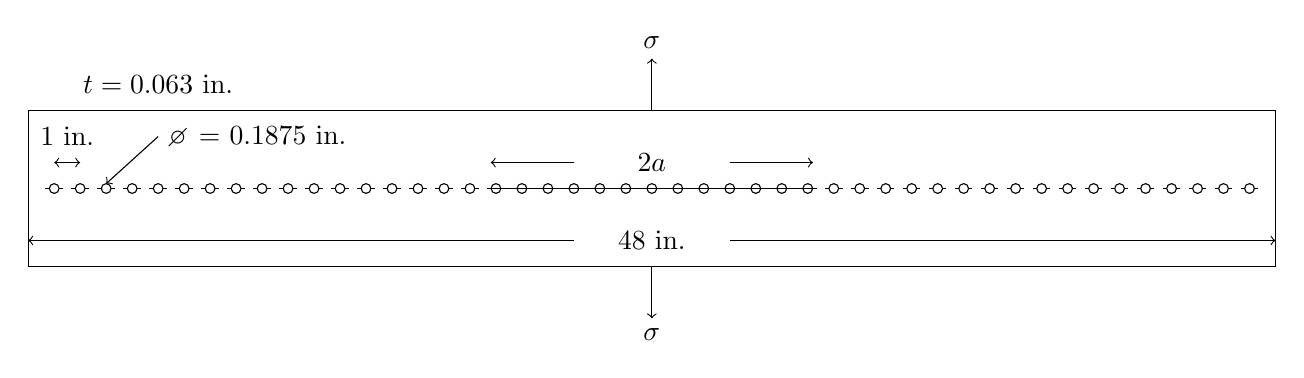
\begin{tikzpicture}
	\begin{scope}[scale=0.33]
	\draw (0,-3) -- (0,3) -- (48,3) -- (48,-3) -- (0,-3);
	\draw[->] (24,3) -- (24,5) node[above] {$\sigma$};
	\draw[->] (24,-3) -- (24,-5) node[below] {$\sigma$};
	\foreach \x in {1,2,...,47} {%
		\draw (\x-.1875-.15,0) -- (\x-.1875,0);
		\draw (\x+.1875+.15,0) -- (\x+.1875,0);
		\draw (\x,0) circle (0.1875);
	};
	\draw (17.8,0) -- (30.2,0);
	\draw[->] (21,1) -- (17.8,1);
	\draw[->] (27,1) -- (30.2,1);
	\draw node at (24,1) {$2a$};
	\draw[->] (21,-2) -- (0,-2);
	\draw[->] (27,-2) -- (48,-2);
	\draw node at (24,-2) {48 in.};
	\draw[<->] (1,1) -- (2,1);
	\draw node at (1.5,2) {1 in.};
	\draw[<-] (3,0.1875) -- (5,2) node[right] {$\diameter$ = 0.1875 in.};
	\draw node at (5,4) {$t=0.063$ in.};
	\end{scope}
	\end{tikzpicture}
\end{figure}

%panel under combined tensile and shear loading
\begin{figure}[H]
	\item For the following panel assume $K_{IC} = 60 \text{ ksi}\sqrt{\text{in}}$ and $a = 0.5 \text{ in}$.
	\begin{enumerate}
		\item Determine the critical values of $\sigma$ and $\tau$ as well as the crack extension angle using the maximum circumferential stress criterion.
		\item Determine the critical values of $\sigma$ and $\tau$ as well as the crack extension angle using the principal stress criterion.
	\end{enumerate}
	\textbf{Note:} Assume $\beta = \beta^\prime = 1$
	
	\centering
	\begin{tikzpicture}
	\draw (0,-2) -- (0,2) -- (4,2) -- (4,-2) -- (0,-2);
	\draw (1.5,0) -- (2.5,0);
	\draw[->] (2,2.5) -- (2,3.5) node[above] {$\sigma = 5\tau$};
	\draw[->] (2,-2.5) -- (2,-3.5) node[below] {$\sigma = 5\tau$};
	\draw[->] (1,2.2) -- (3,2.2);
	\draw[->] (3,-2.2) -- (1,-2.2);
	\draw[->] (4.2,-1) -- (4.2,1);
	\draw[->] (-0.2,1) -- (-0.2,-1);
	\draw node at (4.2,2.2) {$\tau$};
	\draw node at (-0.2,-2.2) {$\tau$};
	\draw node at (2,0.2) {$2a$};
	\end{tikzpicture}
\end{figure}

%cantilever beam from homework 1 (consider effects of mode I and mode II)
\begin{figure}[H]
	\item An aluminum beam has a 0.3" crack in the upper flange as shown. 
	Estimate the mixed-mode stress intensity factor.
	
	\textbf{Note:} Assume $K_{II} = \tau \sqrt{\pi a}$.
	
	\centering
	\begin{minipage}{0.7\textwidth}
		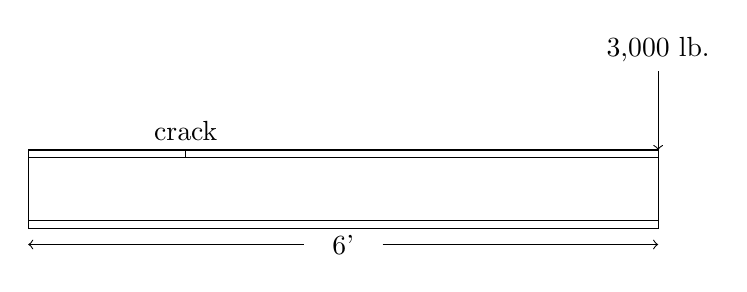
\begin{tikzpicture}
		\point{a}{0}{0};
		\draw (0,-0.5) -- (0,0.5) -- (8,0.5) -- (8,-0.5) -- (0,-0.5);
		\support{3}{a}[-90];
		\draw[->] (8,1.5) node[above] {3,000 lb.}--(8,0.5);
		\draw (0,0.4) -- (8,0.4);
		\draw (0,-0.4) -- (8,-0.4);
		\draw (2,0.5) node[above] {crack} -- (2,0.4);
		\draw[<-] (0,-0.7) -- (3.5,-0.7);
		\draw node at (4,-0.7) {6'};
		\draw[->] (4.5,-0.7) -- (8,-0.7);
		\end{tikzpicture}	
	\end{minipage}
	\begin{minipage}{0.25\textwidth}
		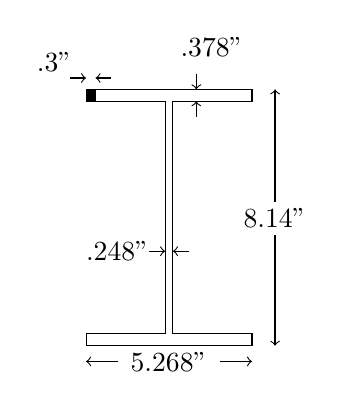
\begin{tikzpicture}
		\begin{scope}[scale=0.4]
		\draw (0,0) -- (5.268,0) -- (5.268, .378) -- (2.758,.378) -- (2.758, 7.762) -- (5.268, 7.762) -- (5.268, 8.14) -- (0,8.14) -- (0,7.762) -- (2.51,7.762) -- (2.51,.378) -- (0,.378) -- (0,0);
		\draw[fill=black] (0.3, 8.14) -- (0,8.14) -- (0,7.762) -- (0.3,7.762);
		\draw node at (2.634,-0.5) {5.268"};
		\draw[->] (1,-0.5) -- (0,-0.5);
		\draw[->] (4.268,-0.5) -- (5.268,-0.5);
		\draw node at (6,4.07) {8.14"};
		\draw[->] (6,3.507) -- (6,0);
		\draw[->] (6,4.57) -- (6,8.14);
		\draw node at (1,3) {.248"};
		\draw[->] (2,3) -- (2.51,3);
		\draw[->] (3.268,3) -- (2.758,3);
		\draw node at (4,9.5) {.378"};
		\draw[->] (3.5,8.64) -- (3.5,8.14);
		\draw[->] (3.5,7.262) -- (3.5,7.762);
		\draw node at (-1,9) {.3"};
		\draw[->] (-0.5,8.5) -- (0,8.5);
		\draw[->] (0.8,8.5) -- (0.3,8.5);
		\end{scope}
		\end{tikzpicture}
	\end{minipage}
	%\caption{Drawing for Problem 5}
\end{figure}

\end{enumerate}
\end{document}
